\chapter*{Programme officiel}

\section*{Programme officiel}

Toute machine informatique manipule une représentation des données dont l'unité minimale est le bit 0/1, ce qui permet d'unifier logique et calcul. Les données de base sont représentées selon un codage dépendant de leur nature : entiers, flottants, caractères et chaînes de caractères. Le codage conditionne la taille des différentes valeurs en mémoire.

{\centering\begin{tabular}{|L{3cm}|L{5.5cm}|L{6cm}|}\hline
\cellcolor{bo}\bfseries\textcolor{white}{Contenus}&
\cellcolor{bo}\bfseries\textcolor{white}{Capacités attendues}&
\cellcolor{bo}\bfseries\textcolor{white}{Commentaires}\\ \hline
Écriture d'un entier positif dans une base $b \geqslant 2$
&
Passer de la représentation d'une base dans une autre.
&
Les bases 2, 10 et 16 sont privilégiées.\\ \hline
Représentation binaire d'un entier relatif
&
Évaluer le nombre de bits nécessaires à l'écriture en base 2 d'un entier, de la somme ou du produit de deux nombres entiers.

Utiliser le complément à 2.
&
Il s'agit de décrire les tailles courantes des entiers (8, 16, 32 ou 64 bits).

Il est possible d'évoquer la représentation des entiers de taille arbitraire de Python.\\ \hline
Représentation approximative des nombres réels : notion de nombre flottant
&
Calculer sur quelques exemples la représentation de nombres réels : \np{0.1}, \np{0.25} ou $1/3$.
&
 $\np{0.2} + \np{0.1}$ n'est pas égal à  \np{0.3}.
 
Il faut éviter de tester l'égalité de deux flottants.

Aucune connaissance précise de la norme IEEE-754 n'est exigible.\\ \hline
Valeurs booléennes : 0, 1. Opérateurs booléens : and, or, not.

Expressions booléennes
&
Dresser la table d'une expression booléenne.
&
Le ou exclusif (xor) est évoqué.

Quelques applications directes comme l'addition binaire sont présentées.

L'attention des élèves est attirée sur le caractère séquentiel de certains opérateurs booléens.\\ \hline
Représentation d'un texte en machine.

Exemples des encodages ASCII, ISO-8859-1, Unicode
&
Identifier l'intérêt des différents systèmes d'encodage.

Convertir un fichier texte dans différents formats d'encodage.
&
Aucune connaissance précise des normes d'encodage n'est exigible.\\ \hline
\end{tabular}\par}


\chapter{Représentation des nombres}

\section{Codage des entiers naturels}

La première règle pour savoir compter est d'être capable de donner l'entier suivant n'importe quel autre. En partant de 0 cela donne :

\begin{multicols}{3}\small\centering
\begin{tabular}{ccc}
$b=2$ &  $10$ & $16$ \\
\hline
\texttt{0} & 0 & \texttt{0} \\
\texttt{1} & 1 & \texttt{1} \\
\texttt{10} & 2 & \texttt{2} \\
\texttt{11} & 3 & \texttt{3} \\
\texttt{100} & 4 & \texttt{4} \\
\texttt{101} & 5 & \texttt{5} \\
\texttt{110} & 6 & \texttt{6} \\
\texttt{111} & 7 & \texttt{7} \\
\texttt{1000} & 8 & \texttt{8} \\
\texttt{1001} & 9 & \texttt{9} \\
\texttt{1010} & 10 & \texttt{A} \\
\texttt{1011} & 11 & \texttt{B} \\
\texttt{1100} & 12 & \texttt{C} \\
\texttt{1101} & 13 & \texttt{D} \\
\texttt{1110} & 14 & \texttt{E} \\
\texttt{1111} & 15 & \texttt{F} \\
\end{tabular}

\begin{tabular}{ccc}
$b=2$ &  $10$ & $16$ \\
\hline
\texttt{1}\,\texttt{0000} & 16 & \texttt{10} \\
\texttt{1}\,\texttt{0001} & 17 & \texttt{11} \\
\texttt{1}\,\texttt{0010} & 18 & \texttt{12} \\
\texttt{1}\,\texttt{0011} & 19 & \texttt{13} \\
\texttt{1}\,\texttt{0100} & 20 & \texttt{14} \\
\texttt{1}\,\texttt{0101} & 21 & \texttt{15} \\
\texttt{1}\,\texttt{0110} & 22 & \texttt{16} \\
\texttt{1}\,\texttt{0111} & 23 & \texttt{17} \\
\texttt{1}\,\texttt{1000} & 24 & \texttt{18} \\
\texttt{1}\,\texttt{1001} & 25 & \texttt{19} \\
\texttt{1}\,\texttt{1010} & 26 & \texttt{1A} \\
\texttt{1}\,\texttt{1011} & 27 & \texttt{1B} \\
\texttt{1}\,\texttt{1100} & 28 & \texttt{1C} \\
\texttt{1}\,\texttt{1101} & 29 & \texttt{1D} \\
\texttt{1}\,\texttt{1110} & 30 & \texttt{1E} \\
\texttt{1}\,\texttt{1111} & 31 & \texttt{1F} \\
\end{tabular}

\begin{tabular}{ccc}
$b=2$ &  $10$ & $16$ \\
\hline
\texttt{10}\,\texttt{0000} & 32 & \texttt{20} \\
\texttt{10}\,\texttt{0001} & 33 & \texttt{21} \\
\texttt{10}\,\texttt{0010} & 34 & \texttt{22} \\
\texttt{10}\,\texttt{0011} & 35 & \texttt{23} \\
\texttt{10}\,\texttt{0100} & 36 & \texttt{24} \\
\ldots & \ldots & \ldots \\
\texttt{1111}\,\texttt{0110} & 246 & \texttt{F6} \\
\texttt{1111}\,\texttt{0111} & 247 & \texttt{F7} \\
\texttt{1111}\,\texttt{1000} & 248 & \texttt{F8} \\
\texttt{1111}\,\texttt{1001} & 249 & \texttt{F9} \\
\texttt{1111}\,\texttt{1010} & 250 & \texttt{FA} \\
\texttt{1111}\,\texttt{1011} & 251 & \texttt{FB} \\
\texttt{1111}\,\texttt{1100} & 252 & \texttt{FC} \\
\texttt{1111}\,\texttt{1101} & 253 & \texttt{FD} \\
\texttt{1111}\,\texttt{1110} & 254 & \texttt{FE} \\
\texttt{1111}\,\texttt{1111} & 255 & \texttt{FF} \\
\end{tabular}
\end{multicols}

\begin{center}
<< Il n'y a que 10 sortes de personnes : celles qui savent compter en binaire et les autres ! >>
\end{center}

\subsection{Lire un entier naturel écrit en base 2 ou 16}

{\bfseries En base 10} : les chiffres ont chacun une signification selon leur position. 

$125 =$
\begin{tabular}{ccc}
centaines & dizaines & unités \\
\hline
1 & 2 & 5\\
\end{tabular}$=$\begin{tabular}{ccc}
$10^2$ & $10^1$ & $10^0$ \\
\hline
1 & 2 & 5\\
\end{tabular} $=1\times10^2+2\times10^1+5\times10^0=125$

{\bfseries En base 2} : $\texttt{11001}_2=$ \begin{tabular}{ccccc}
 $2^4$ & $2^3$ & $2^2$ & $2^1$ & $2^0$ \\
\hline
\texttt{1} & \texttt{1} & \texttt{0} &\texttt{0} & \texttt{1} \\
\end{tabular} $=1\times2^4+1\times2^3+0\times2^2+0\times2^1+1\times2^0=25$

De tête, on calcule d'abord les puissances : $\texttt{11001}_2=$ \begin{tabular}{ccccc}
 $16$ & $8$ & $4$ & $2$ & $1$ \\
\hline
\texttt{1} & \texttt{1} & \texttt{0} &\texttt{0} & \texttt{1} \\
\end{tabular} $=16+8+1=25$

À la machine, on évite les puissances : $\texttt{11001}_2=(((1 \times 2+ 1) \times 2 +0)\times 2 + 0)\times2+1 =25$ 

{\bfseries En base 16} : $\texttt{C9}_{16}=$ \begin{tabular}{cc}
$16^1$ & $16^0$ \\
\hline
\texttt{12} & \texttt{9} \\
\end{tabular} $=12\times16+9=81$

Les trois écritures sont utilisables avec Python : \pythoninline{0b11001} vaut 25 et \pythoninline{0xC9} vaut 81.

\subsection{Écrire un entier naturel en base 2 ou 16}

\subsubsection{De la base 10 vers la base 2} On part de l'astuce de factorisation vue plus haut :

\begin{tabular}{c@{\,$=$\,}c@{\,$\times$\,}lll}
$25$ & $12$ & $2 + 1$ & donc & $25=12\times2 + 1  = \texttt{?...?1}_2$\\

$12$ & $6$ & $2 + 0$ & donc & $25=(6\times2+0)\times2 + 1  = \texttt{?...?01}_2$\\

$6$ & $3$ & $2 + 0$ & donc & $25=((3\times2+0)\times2+0)\times2 + 1  = \texttt{?...?001}_2$\\

$3$ & $1$ & $2 + 1$ & donc & $25=(((1\times2+1)\times2+0)\times2+0)\times2 + 1  = \texttt{?...?1001}_2$\\

$1$ & $0$ & $2 + 1$ & donc & $25=(((1\times2+1)\times2+0)\times2+0)\times2 + 1  = \texttt{11001}_2$\\
\end{tabular}

On vient de procéder par divisions euclidiennes par 2 successives, jusqu'à trouver un quotient nul. L'écriture binaire est la succession des restes trouvés (à l'envers).

Avec Python : \pythoninline{bin(25)} donne bien \pythoninline{'0b11001'}.

\medskip

\subsubsection{De la base 10 vers la base 16} On peut procéder de même par division euclidienne par 16.

\begin{tabular}{c@{\,$=$\,}c@{\,$\times$\,}lll}
$2019$ & $126$ & $16 + 3$ & donc & $2019=126\times16 + 3  = \texttt{?...?3}_{16}$\\

$126$ & $7$ & $16 + 14$ & donc & $2019=(7\times16+14)\times16 + 3  = \texttt{?...?E3}_{16}$\\

$7$ & $0$ & $16 + 7$ & donc & $2019=(7\times16+14)\times16 + 3  = \texttt{7E3}_{16}$\\
\end{tabular}

Avec Python : \pythoninline{hex(2019)} donne bien \pythoninline{'0x7e3'}.

\subsubsection{De la base 2 vers la base 16} On fait des paquets de 4 !

$\texttt{1011\,0110}_2
=1\times2^7+0\times2^6+1\times2^5+1\times2^4+0\times2^3+1\times2^2+1\times2^1+0\times2^0$

$\texttt{1011\,0110}_2
=(1\times2^3+0\times2^2+1\times2^1+1\times2^0)\times2^4+(0\times2^3+1\times2^2+1\times2^1+0\times2^0)$

\fbox{$\texttt{1011\,0110}_2=\texttt{1011}_2\times 16 +\texttt{0110}_2$}

$\texttt{1011\,0110}_2=\texttt{B}_{16}\times 16 +\texttt{6}_{16}$

$\texttt{1011\,0110}_2=\texttt{B6}_{16}$

Avec Python : \pythoninline{hex(0b10110110)} donne bien \pythoninline{'0xb6'}.

\section{Codage des entiers relatifs}

\subsection{Recours au bit de signe}

Pour représenter les entiers relatifs en binaire, la première démarche est de réserver un bit pour coder son signe.

\begin{itemize}
	\item \tikz[baseline=(O.base)]\node[circle, inner sep=1pt, draw,fill=black!5](O){\texttt{0}};\!\texttt{101\,1101} est un entier positif (premier bit à gauche égal à 0)
	\item \tikz[baseline=(O.base)]\node[circle, inner sep=1pt, draw,fill=black!5](O){\texttt{1}};\!\texttt{101\,1101} est un entier négatif (premier bit à gauche égal à 1)
\end{itemize}

\medskip

Le bit de signe étant à gauche il convient de normaliser la taille du mot binaire représentant ces entiers. On utilise généralement 8, 16, 32 ou 64 bits (1, 2, 4 ou 8 octets).

Pour simplifier les explications dans ce cours, on les représentera sur 4 bits seulement, mais on ne perd pas en généralité.

\medskip

On peut alors se servir du reste des bits pour coder l'entier naturel correspondant.

Si l'entier est positif on retrouve le codage d'un entier naturel :

\begin{center}
\begin{tabular}{cccccccc}
0 &1 &2 &3 &4 &5 &6 &7 \\ \hline
\texttt{0000} &\texttt{0001} &\texttt{0010} &\texttt{0011} &\texttt{0100} &\texttt{0101} &\texttt{0110} &\texttt{0111}\\
\end{tabular}\end{center}

mais si on utilise le même raisonnement pour coder les nombres négatifs, on se heurte à différents problèmes :



\begin{center}
\begin{tabular}{cccccccc}
$-0$ ? &$-1$ ? &$-2$ ? &$-3$ ? &$-4$ ? &$-5$ ? &$-6$ ? &$-7$ ? \\ \hline
\texttt{1000} &\texttt{1001} &\texttt{1010} &\texttt{1011} &\texttt{1100} &\texttt{1101} &\texttt{1110} &\texttt{1111}\\
\end{tabular}\end{center}

\begin{itemize}
	\item \texttt{1000} voudrait dire $-0$ donc on aurait deux représentations différentes de 0.
	\item Ajouter 1 au nombre binaire ferait diminuer l'entier négatif de 1 !
\end{itemize}

On a donc opté pour le codage suivant :
\begin{center}
\begin{tabular}{cccccccc}
$-8$ &$-7$ &$-6$ &$-5$ &$-4$ &$-3$ &$-2$ &$-1$ \\ \hline
\texttt{1000} &\texttt{1001} &\texttt{1010} &\texttt{1011} &\texttt{1100} &\texttt{1101} &\texttt{1110} &\texttt{1111}\\
\end{tabular}\end{center}

On peut en donner une représentation circulaire :

\begin{center}
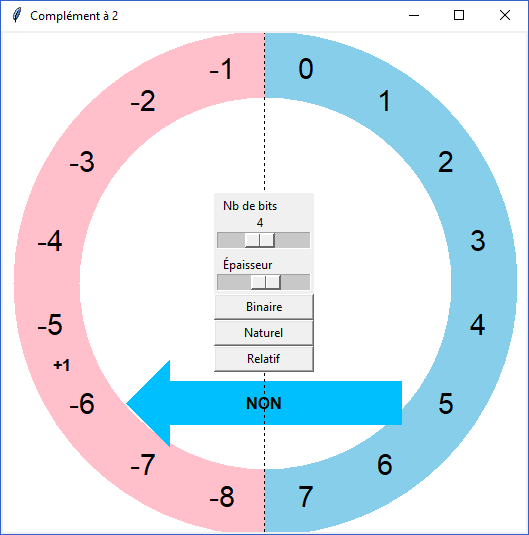
\includegraphics[scale=0.33]{images/complementa2rel.png}\quad
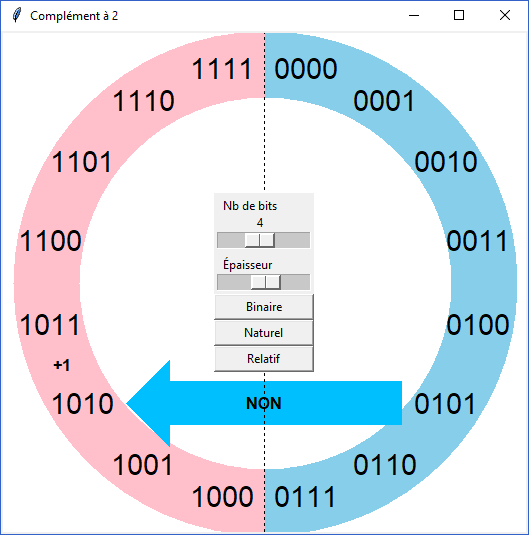
\includegraphics[scale=0.33]{images/complementa2bin.png}
\end{center}

Les nombres binaires et les nombres relatifs sont écrits dans l'ordre en tournant dans le sens des aiguilles d'une montre, tout en conservant la signification du bit de signe. 

Comme on n'a pas de << $-0$ >> il y a un décalage de 1 dans la symétrie entre entiers positifs et négatifs alors qu'elle est parfaite pour les binaires.

\subsection{Complément à 2}

Les résultats précédents permettent de dégager une méthode de codage  :

\begin{center}
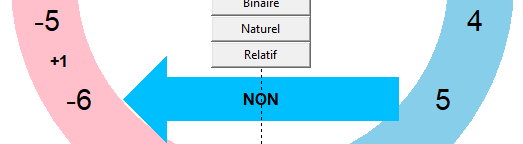
\includegraphics[scale=0.45]{images/complementa2relzoom.png}\quad
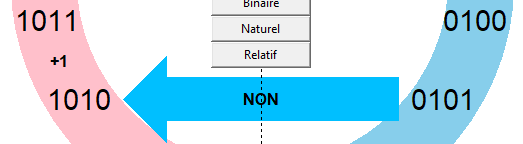
\includegraphics[scale=0.45]{images/complementa2binzoom.png}
\end{center}

Pour coder un entier négatif ($-5$) par complément à 2 sur $n$($=4$) bits, 

\begin{center}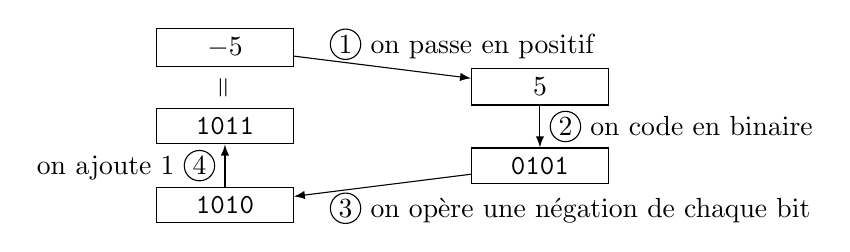
\begin{tikzpicture}
\node[draw, text width = 1.5cm,align = center](N)at(-2,2){$-5$};
\node[draw, text width = 1.5cm,align = center](P)at(2,1.5){$5$};
\draw[-latex](N)--(P)node[pos = 0.2, above right, inner sep = 0]{\tikz[baseline=(O.base)]\node[inner sep = 1pt,circle,draw](O){1}; on passe en positif};
\node[draw, text width = 1.5cm,align = center](B1)at(2,0.5){\texttt{0101}};
\draw[-latex](P)--(B1)node[midway, right]{\tikz[baseline=(O.base)]\node[inner sep = 1pt,circle,draw](O){2}; on code en binaire};
\node[draw, text width = 1.5cm,align = center](B2)at(-2,0){\texttt{1010}};
\draw[-latex](B1)--(B2)node[pos = 0.8, below right, inner sep = 0]{\tikz[baseline=(O.base)]\node[inner sep = 1pt,circle,draw](O){3}; on opère une négation de chaque bit};
\node[draw, text width = 1.5cm,align = center](B3)at(-2,1){\texttt{1011}};
\draw[-latex](B2)--(B3)node[midway, left]{on ajoute 1 \tikz[baseline=(O.base)]\node[inner sep = 1pt,circle,draw](O){4};};
\path(B3)--(N)node[midway,sloped]{$=$}; 
\end{tikzpicture}\end{center}

Pour décoder un nombre binaire (\texttt{1011}), on peut suivre un cycle similaire :

\begin{center}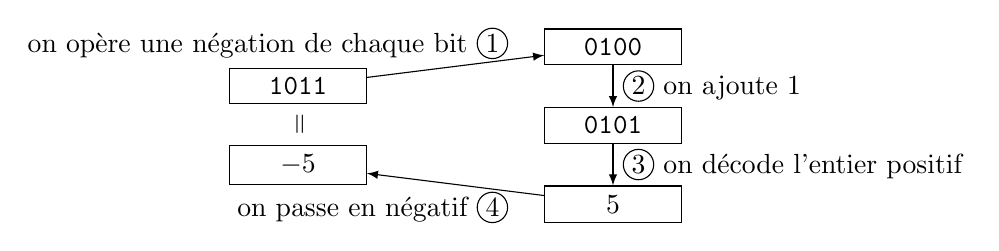
\begin{tikzpicture}
\node[draw, text width = 1.5cm,align = center](B1)at(-2,1.5){\texttt{1011}};
\node[draw, text width = 1.5cm,align = center](B2)at(2,2){\texttt{0100}};
\draw[-latex](B1)--(B2)node[pos = 0.8,above left, inner sep = 0]{on opère une négation  de chaque bit \tikz[baseline=(O.base)]\node[inner sep = 1pt,circle,draw](O){1};};
\node[draw, text width = 1.5cm,align = center](B3)at(2,1){\texttt{0101}};
\draw[-latex](B2)--(B3)node[midway, right]{\tikz[baseline=(O.base)]\node(O)[inner sep = 1pt,circle,draw]{2}; on ajoute 1};
\node[draw, text width = 1.5cm,align = center](P)at(2,0){$5$};
\draw[-latex](B3)--(P)node[midway, right]{\tikz[baseline=(O.base)]\node[inner sep = 1pt,circle,draw](O){3}; on décode l'entier positif};
\node[draw, text width = 1.5cm,align = center](N)at(-2,0.5){$-5$};
\draw[-latex](P)--(N)node[pos = 0.2, below left, inner sep = 0]{on passe en négatif \tikz[baseline=(O.base)]\node[inner sep = 1pt,circle,draw](O){4};};
\path(B1)--(N)node[midway,sloped]{$=$}; 
\end{tikzpicture}\end{center}

En fait, pour coder l'entier $-5$, on cherche le nombre $n$ qui vérifie $n+5=0$

\begin{center}\begin{tabular}{cccccl}
{\footnotesize {\footnotesize $1$}} & {\footnotesize $1$} & {\footnotesize $1$} & {\footnotesize $1$} &  & {\footnotesize $\leftarrow$ retenues}\\
 & $0$ & $1$ & $0$ & $1$ &  $\leftarrow 5$\\
$+$ & $1$ & $0$ & $1$ & $1$ & $\leftarrow -5$\\
\cline{1-5}
$(1)$ & $0$ & $0$ & $0$ & $0$ & $\leftarrow 16=2^4$\\
\end{tabular}\end{center}

D'un point de vue des écritures binaires, cela revient à provoquer une retenue qui dépasse le nombre $n$ de bits de l'écriture pour n'obtenir (lui mis à part) que des bits à 0 : on cherche le nombre $n$ qui vérifie $n+5=2^4$ c'est à dire le complément de $5$ à $2^4$.

\Cours{{\bfseries Complément à 2}

L'écriture d'un nombre binaire négatif $m$ en complément à 2 sur $n$ bits est l'écriture binaire du nombre positif $p$ tel que $p + (-m) = 2^n$, c'est à dire, le complément à $2^n$ de $-m$.
}

\subsection{Nombre de bits nécessaires aux opérations}

Un nombre codé sur $n$ bits peut s'écrire de $2^n$ façons. $n$ bits permettent donc de coder 
 tous les {\bfseries entiers naturels} de $\texttt{00...0}_{2}=0$ à $\texttt{11...1}_{2}=2^n-1$.

\begin{center}
\begin{tabular}{ccc}
codage en & plus grand entier  & exemple\\
\hline
8 bits  = 1 octet & \np{255} & primaire RVB \\
16 bits  = 2 octets & \np{65535} & \\
24 bits  = 3 octets & \np{16777215} & couleur RVB \\
32 bits  = 4 octets & \np{4294967295} & IPv4\\
64 bits  = 8 octets & \np{18446744073709551615} & SE actuels \\
\end{tabular}
\end{center}

	Comme $1_2=2^0$, $10_2=2^1$, $100_2=2^2$, $1000_2=2^3$, $10000_2=2^4$, ... 
	
	\begin{center}
	
	Un nombre $n$ a au plus $k$ bits significatifs si et seulement si $n < 2^k$.
	
	\end{center}
	
	({\bfseries Pour aller plus loin : } Il existe une fonction mathématique définissant le réel $y$ tel que $n = 2^y$. Il s'agit de $\text{log}_2$, le logarithme à base 2 : $n = 2^{\text{log}_2(n)}$.)
	
	\begin{itemize}
		\item Additionner deux entiers naturels $n$ et $p$ avec au plus $k$ bits significatifs en nécessite au plus $k+1$ (en effet :  $n < 2^k$ et  $p < 2^k$ donnent  $n + p < 2^k + 2^k = 2\times 2^k = 2^{k+1}$)
		
		(Ce << $+1$ >> correspondant à une éventuelle retenue.)
		\item Multiplier deux entiers naturels $n$ et $p$ avec respectivement au plus $k$ et $l$ bits significatifs en nécessite au plus $k+l$ (en effet :  $n < 2^k$ et  $p < 2^l$ donnent  $n \times p < 2^k \times 2^l = 2^{k+l}$)
	\end{itemize}
	
	\medskip
	
	Un nombre codé sur $n$ bits peut s'écrire de $2^n$ façons. $n$ bits permettent donc de coder 
 tous les {\bfseries entiers relatifs} de $\texttt{10...0}_{2}=-2^{n-1}$ à $\texttt{01...1}_{2}=-2^{n-1}-1$.

\begin{center}
\begin{tabular}{ccc}
codage en & plus petit entier & plus grand entier \\
\hline
8 bits  =  1 octet & \np{-128} & \np{127} \\
16 bits  = 2 octets & \np{-32768} & \np{32 767}\\
32 bits  = 4 octets & \np{-2147483648} & \np{2147483647}\\
64 bits = 8 octets & \np{-9223372036854775808} & \np{9223372036854775807} \\
\end{tabular}
\end{center}

	\begin{itemize}
		\item Additionner un négatif avec un positif ne pose jamais de problème.
		\item Ajouter deux positifs trop grands risque de donner un résultat négatif.
		
		(la retenue se déportant sur le bit de signe.)
		\item Ajouter deux négatifs trop grands risque de donner un résultat positif (même raison).
	\end{itemize}
	
	Il est difficile de mettre en évidence ces dépassements avec Python qui définit des entiers de taille arbitraire. On peut en avoir un aperçu avec la calculatrice de windows en mode programmeur, si on essaie de calculer $\np{9223372036854775807}+1$ on trouve $\np{-9223372036854775808}$, les entiers relatifs étant codés sur 64 bits.

\section{Codage des << réels >>}

Les nombres irrationnels (comme $\sqrt{2}$ ou $\pi$) \emph{ne} peuvent \emph{pas} être représentés car ils contiennent une infinité de chiffres significatifs sans répétition pour les décrire. Et même si c'était possible, n'importe quel intervalle, aussi petit soit-il, contient une infinité de réels donc impossible à distinguer avec un nombre fini de bits. Tout ce que l'on peut faire, c'est coder quelques nombres rationnels choisis.

\subsection{Codage en virgule flottante}

{\bfseries L'écriture décimale} d'un nombre se fait en deux parties finies séparées par une virgule. Par exemple : $\np{324.125} = 3\times 10^2 + 2\times 10^1 + 4\times 10^0 + 1\times 10^{-1} + 2\times 10^{-2} + 5\times 10^{-3}$.

On peut utiliser la même notation en binaire : 

$\np{101.001}_2 = 1\times 2^2 + 0\times 2^1 + 1\times 10^0  + 0\times 2^{-1} + 0\times 2^{-2} + 1\times 2^{-3} (= \np{5.125})$

\medskip

{\bfseries L'écriture scientifique} permet de standardiser l'écriture décimale : $\np{324.125} = \np{3.24125}\times 10^2$

L'avantage pour un nombre binaire ($\neq0$), est que le premier chiffre est toujours 1. Par exemple $101,001_2 = 1,01001_2 \times 10_2\,^{10_2}$. On parle d'écriture normalisée. Il suffit donc de se souvenir de la mantisse (chiffres après la virgule) et de l'exposant. Sans entrer plus dans les détails, voilà comment on procède :

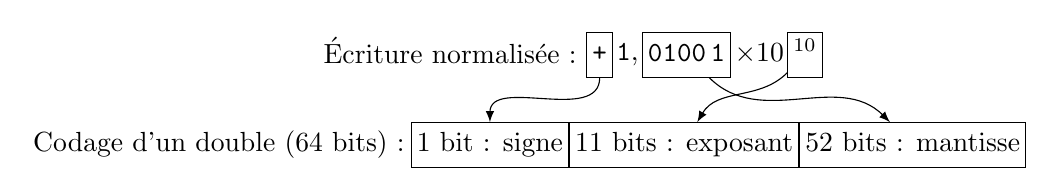
\begin{tikzpicture}[scale=0.5]
\node[](N){\strut Écriture normalisée :~};
\node[draw, right, inner sep = 2pt](S)at(N.east){\strut\texttt{+}};
\node[right, inner sep = 1pt](U)at(S.east){\texttt{1},};
\node[draw, right, inner sep = 2pt](M)at(U.east){\strut\texttt{0100}\,\texttt{1}};
\node[right, inner sep = 1pt](P)at(M.east){\strut $\times 10$};
\node[draw, right, inner sep = 2pt](E)at(P.east){\strut $^{10}$};
%
\node[below left=0.5cm, inner sep = 2pt](C)at(N.south){\strut Codage d'un double (64 bits) :~};
\node[draw, right, inner sep = 2pt](CS)at(C.east){\strut 1 bit : signe};
\node[draw, right, inner sep = 2pt](CE)at(CS.east){\strut 11 bits : exposant};
\node[draw, right, inner sep = 2pt](CM)at(CE.east){\strut 52 bits : mantisse};
%
\draw[-latex](S)to[out=-90, in=90](CS);
\draw[-latex](M)to[out=-45, in=135](CM);
\draw[-latex](E)to[out=-135, in=60](CE);
\end{tikzpicture}

\subsection{Problème d'arrondis}

On peut coder la partie décimale d'un nombre par soustractions successives des puissances de 2 d'exposant négatifs :

\begin{tabular}{c@{\,$=$\,}c@{\,$+$\,}l@{\, donc : \,}l}
$\np{0.625}$ & $\np{0.125}$ & $1\times2^{-1}$ & $\np{0.625}= \texttt{0,1?...}_2$\\

$\np{0.125}$ & $\np{0.125}$ & $0\times2^{-2}$ & $\np{0.625}= \texttt{0,10?...}_2$\\

$\np{0.125}$ & $0$ & $1\times2^{-3}$ & $\np{0.625}= \texttt{0,101}_2$\\
\end{tabular}

Si on essaie de déterminer l'écriture binaire de \np{0.1} :

\begin{tabular}{c@{\,$=$\,}c@{\,$+$\,}l@{\, donc : \,}l}
$\np{0.1}$ & $\np{0.0375}$ & $1\times2^{-4}$ & $\np{0.1}= \texttt{0,0001?...}_2$\\

$\np{0.0375}$ & $\np{0.00625}$ & $1\times2^{-5}$ & $\np{0.1}= \texttt{0,00011?...}_2$\\

$\np{0.00625}$ & $\np{0.00625}$ & $0\times2^{-6}$ & $\np{0.1}= \texttt{0,000110?...}_2$\\

$\np{0.00625}$ & $\np{0.00625}$ & $0\times2^{-7}$ & $\np{0.1}= \texttt{0,0001100?...}_2$\\

$\np{0.00625}$ & $\np{0,00234375}$ & $1\times2^{-8}$ & $\np{0.1}= \texttt{0,00011001?...}_2$\\

$\np{0,00234375}$ & $\np{0,000390625}$ & $1\times2^{-9}$ & $\np{0.1}= \texttt{0,000110011?...}_2$\\

$\np{0,000390625}$ & $\np{0,000390625}$ & $0\times2^{-10}$ & $\np{0.1}= \texttt{0,0001100110?...}_2$\\

$\np{0,000390625}$ & $\np{0,000390625}$ & $0\times2^{-11}$ & $\np{0.1}= \texttt{0,00011001100?...}_2$\\

$\np{0,000390625}$ & $\np{0,000146484375}$ & $1\times2^{-12}$ & $\np{0.1}= \texttt{0,000110011001?...}_2$\\
\end{tabular}

... $\np{0.1}= \texttt{0,0001100110011001100110011001100110011001100110011001100110011...}_2$

Donc \np{0.1} \emph{n'}est \emph{pas} représentable par le codage binaire en virgule flottante !

L'écriture en Python : \pythoninline{x = 0.1} fait donc un arrondi (56 bits après la virgule).

Il n'est donc pas étonnant d'obtenir des résultats approchés par ce codage :

\pythoninline{print(0.1 + 0.2)} affiche \pythoninline{0.30000000000000004}

\pythoninline{print(0.1 + 0.2 == 0.3)} affiche \pythoninline{False}

Ce n'est donc \emph{jamais} une bonne idée de faire des tests d'égalité avec des nombres à virgules flottantes. On préfèrera toujours, quand c'est possible, utiliser des entiers.



\chapter{Expressions booléennes}

\section{Valeurs booléennes}
L'ensemble des booléens comporte exactement deux valeurs : << vrai >> ou << faux >>.

Le type \pythoninline{bool} de Python les note \pythoninline{True} et \pythoninline{False}.

Les variables booléennes servent aux instructions conditionnelles.

\begin{multicols}{2}
\begin{minted}{python3}
if test :
    print('Le test est vrai')
else :
    print('Le test est faux')
\end{minted}  


\begin{minted}{python3}
while test :
    print('Le test est vrai')
    fait_un_truc()
\end{minted}  
\end{multicols}

Les autres types peuvent aussi être évalués comme un booléen :

\begin{minted}{python3}
for test in [True, False, 0, 1, 127, '0', 0.0, 12.34, [], [0], print] :
    if test:
        print(type(test),test,"= vrai.")
    else :
        print(type(test),test,"= faux.")
\end{minted}

\begin{itemize}
	\item {\bfseries FAUX} : \pythoninline{False}, $0$ ou vide.
	\item {\bfseries VRAI} : Tout le reste (ce qui n'est pas faux est vrai).
\end{itemize}

Pour simplifier nous confondrons en particulier \pythoninline{False} avec $0$ et \pythoninline{True} avec $1$.

Dans un souci de lisibilité, on évitera d'écrire des conditionnelles d'un autre type.

\section{Opérateurs booléens}

Comme il n'y a que deux valeurs booléennes, il suffit, pour décrire n'importe quelle fonction ou opérateur booléen, de dresser son tableau de valeurs, appelé : {\bfseries table de vérité}.

\subsection{Une variable}

Il n'existe que $2^2=4$ tables de vérité portant sur une seule variable :

\begin{multicols}{4}

\begin{tabular}{c|cc}
$a$ & \texttt{0} & \texttt{1} \\
\hline
$f_0(a)$ & \texttt{0} & \texttt{0} \\
\end{tabular}


\begin{tabular}{c|cc}
$a$ & \texttt{0} & \texttt{1} \\
\hline
$f_1(a)$ & \texttt{0} & \texttt{1} \\
\end{tabular}


\begin{tabular}{c|cc}
$a$ & \texttt{0} & \texttt{1} \\
\hline
$f_2(a)$ & \texttt{1} & \texttt{0} \\
\end{tabular}


\begin{tabular}{c|cc}
$a$ & \texttt{0} & \texttt{1} \\
\hline
$f_3(a)$ & \texttt{1} & \texttt{1} \\
\end{tabular}

\end{multicols}

$f_0 = 0$ et $f_3 = 1$ et $f_1(a)=a$ n'ont pas besoin d'être nommées pour être utilisées.

$f_2$ par contre permet d'échanger \pythoninline{True} et \pythoninline{False} : c'est une négation.

Python la note \pythoninline{not} et elle s'utilise sans parenthèses. L'équivalent binaire est \pythoninline{~}.

\begin{center}
\begin{tabular}{c|cc}
\pythoninline{a} & \pythoninline{False} & \pythoninline{True} \\
\hline
\pythoninline{not a} & \pythoninline{True} &  \pythoninline{False} \\
\end{tabular} \qquad \qquad
\begin{tabular}{c|cc}
\pythoninline{a} & \pythoninline{0b0} & \pythoninline{0b1} \\
\hline
\pythoninline{~a} & \pythoninline{0b1} &  \pythoninline{0b0} \\
\end{tabular} 
\end{center}

\subsection{Deux variables}

Il existe $2^4=16$ fonctions à 2 variables booléennes. Les trois plus utilisées sont :

\begin{tabular}{c|cccc}
$a$ & \texttt{0} & \texttt{0} & \texttt{1} & \texttt{1} \\
$b$ & \texttt{0} & \texttt{1} & \texttt{0} & \texttt{1} \\
\hline
{\bfseries et}& \texttt{0} & \texttt{0} & \texttt{0} & \texttt{1} \\
\end{tabular} \qquad
\begin{tabular}{c|cccc}
$a$ & \texttt{0} & \texttt{0} & \texttt{1} & \texttt{1} \\
$b$ & \texttt{0} & \texttt{1} & \texttt{0} & \texttt{1} \\
\hline
{\bfseries ou}& \texttt{0} & \texttt{1} & \texttt{1} & \texttt{1} \\
\end{tabular} \qquad
\begin{tabular}{c|cccc}
$a$ & \texttt{0} & \texttt{0} & \texttt{1} & \texttt{1} \\
$b$ & \texttt{0} & \texttt{1} & \texttt{0} & \texttt{1} \\
\hline
{\bfseries ou exclusif}& \texttt{0} & \texttt{1} & \texttt{1} & \texttt{0} \\
\end{tabular}

Python note << et >> : \pythoninline{and} et << ou >> : \pythoninline{or}, mais n'a pas de notation dédiée au << ou exclusif >>. Les équivalents binaires sont respectivement \pythoninline{&}, \pythoninline{|} et \pythoninline{^}.



\begin{center}
\begin{tabular}{c|cccc}
\pythoninline{a} & \pythoninline{False} & \pythoninline{False} & \pythoninline{True} & \pythoninline{True} \\
\pythoninline{a} & \pythoninline{False} & \pythoninline{True} & \pythoninline{False} & \pythoninline{True} \\
\hline
\pythoninline{a and b} & \pythoninline{False} &  \pythoninline{False} & \pythoninline{False} &  \pythoninline{True} \\
\end{tabular} \quad
\begin{tabular}{c|cccc}
\pythoninline{a} & \pythoninline{0b0} & \pythoninline{0b0} & \pythoninline{0b1} & \pythoninline{0b1} \\
\pythoninline{b} & \pythoninline{0b0} & \pythoninline{0b1} & \pythoninline{0b0} & \pythoninline{0b1} \\
\hline
\pythoninline{a & b} & \pythoninline{0b0} &  \pythoninline{0b0} & \pythoninline{0b0} &  \pythoninline{0b1} \\
\end{tabular}

\medskip

\begin{tabular}{c|cccc}
\pythoninline{a} & \pythoninline{False} & \pythoninline{False} & \pythoninline{True} & \pythoninline{True} \\
\pythoninline{a} & \pythoninline{False} & \pythoninline{True} & \pythoninline{False} & \pythoninline{True} \\
\hline
\pythoninline{a or b} & \pythoninline{False} &  \pythoninline{True} & \pythoninline{True} &  \pythoninline{True} \\
\end{tabular} \quad
\begin{tabular}{c|cccc}
\pythoninline{a} & \pythoninline{0b0} & \pythoninline{0b0} & \pythoninline{0b1} & \pythoninline{0b1} \\
\pythoninline{b} & \pythoninline{0b0} & \pythoninline{0b1} & \pythoninline{0b0} & \pythoninline{0b1} \\
\hline
\pythoninline{a | b} & \pythoninline{0b0} &  \pythoninline{0b1} & \pythoninline{0b1} &  \pythoninline{0b1} \\
\end{tabular}

\medskip

\begin{tabular}{c|cccc}
\pythoninline{a} & \pythoninline{0b0} & \pythoninline{0b0} & \pythoninline{0b1} & \pythoninline{0b1} \\
\pythoninline{b} & \pythoninline{0b0} & \pythoninline{0b1} & \pythoninline{0b0} & \pythoninline{0b1} \\
\hline
\pythoninline{a ^ b} & \pythoninline{0b0} &  \pythoninline{0b1} & \pythoninline{0b1} &  \pythoninline{0b0} \\
\end{tabular}
\end{center}

\pythoninline{not}, \pythoninline{and} et \pythoninline{or} sont appelés {\bfseries opérateurs logiques}.

\pythoninline{~}, \pythoninline{&}, \pythoninline{|}, \pythoninline{^} sont des {\bfseries opérateurs  binaires}.

Comme les booléens sont identifiés aux binaires 0 et 1, on peut utiliser  \pythoninline{^}.

\pythoninline{True ^ True} vaut bien \pythoninline{False}, \pythoninline{True ^ False} vaut bien \pythoninline{True}, etc...

Mais il faut faire attention aux priorités de calcul. Le calcul binaire est prioritaire par rapport au calcul booléen. Dans le doute : surcharger de parenthèses ; ne pas mélanger les types ; ou passer par une fonction (dont l'évaluation est encore plus prioritaire mais qui oblige les parenthèses).

\begin{multicols}{2}

On pourra par exemple définir une fonction \pythoninline{xor()} pour les booléens (ci-contre).

\begin{minted}{python3}
def xor(a, b):
    return a ^ b
\end{minted}

\end{multicols}

\section{Caractère séquentiel des opérateurs logiques}

Pour évaluer \pythoninline{a and b}, Python évalue d'abord \pythoninline{a}. 

\begin{itemize}
	\item S'il est \pythoninline{False}, quelque soit \pythoninline{b}, la réponse sera \pythoninline{False}, donc \pythoninline{b} n'est pas évalué.
	
	C'est très pratique, par exemple quand on veut évaluer une valeur d'un tableau :
	
	\pythoninline{if i < len(T) and T[i] > 0 :} si l'indice sort du tableau, \pythoninline{T[i]} ne sera pas évalué.
	
	\item S'il est \pythoninline{True}, \pythoninline{b} détient la réponse : c'est sa valeur qui est renvoyée (sans être testée).
	
	Cela permet un autre raccourci d'écriture : 
	
	\pythoninline{b =  0 <= i < len(T) and T[i]} vaut \pythoninline{False} si \pythoninline{i} sort du tableau et \pythoninline{T[i]} sinon.
\end{itemize}

\begin{multicols}{2}

Grossièrement \pythoninline{a and b} revient à :

\begin{minted}{python3}
def et(a,b):
    if a :
        resultat = b
    else :
        resultat = False
    return resultat
\end{minted}

De même,  \pythoninline{a or b} revient à :

\begin{minted}{python3}
def ou(a,b):
    if a :
        resultat = True
    else :
        resultat = b
    return resultat
\end{minted}

\end{multicols}

On voit en particulier que \pythoninline{a and b} et \pythoninline{b and a} n'ont pas vraiment la même signification (alors que \pythoninline{a & b} et \pythoninline{b & a} si, en binaire)

En utilisant ces deux opérateurs, on arrive parfois à des instructions conditionnelles très courtes (qui ne sont spécialement à rechercher mais à savoir lire) comme :  

\pythoninline{parite = x % 2 == 0 and "pair" or "impair"}


\section{Expressions booléennes}

Une expression booléenne est une expression dont les variables sont booléennes, les opérateurs << non >>,  << ou >> et  << et >> avec éventuellement des parenthèses pour les priorités.

Exemple : \pythoninline{a and not b or not a and b}

Comme toute variable ne peut prendre que 2 valeurs, on peut toujours dresser un tableau de valeurs complet d'une expression booléenne, appelée table de vérité. 

{\bfseries Priorité : } \pythoninline{not} puis \pythoninline{and} puis \pythoninline{or}.

{\centering
\begin{tabular}{c|cccc}
\pythoninline{a} & \texttt{0} & \texttt{0} & \texttt{1} & \texttt{1} \\
\pythoninline{b} & \texttt{0} & \texttt{1} & \texttt{0} & \texttt{1} \\
\hline
\pythoninline{not a} & \texttt{1} & \texttt{1} & \texttt{0} & \texttt{0} \\
\pythoninline{not b} & \texttt{1} & \texttt{0} & \texttt{1} & \texttt{0} \\
\hline
\pythoninline{a and not b} & \texttt{0} & \texttt{0} & \texttt{1} & \texttt{0} \\
\pythoninline{not a and b} & \texttt{0} & \texttt{1} & \texttt{0} & \texttt{0} \\
\hline
\pythoninline{a and not b or not a and b}& \texttt{0} & \texttt{1} & \texttt{1} & \texttt{0} \\
\end{tabular}\par}

Donc \pythoninline{a and not b or not a and b} est une  expression booléenne du << ou exclusif >>.

\medskip

Les {\bfseries règles de calculs} (pour \pythoninline{a} et \pythoninline{b} booléens) :

\begin{multicols}{2}\begin{itemize}
	\item Associativité : 
	
	\pythoninline{(a or b) or c} =  \pythoninline{a or (b or c)}
	
	\pythoninline{(a and b) and c} = \pythoninline{a and (b and c)}
    \item Commutativité : 
    
    \pythoninline{a or b} = \pythoninline{b or a}
    
    \pythoninline{a and b} = \pythoninline{b and a}
    \item Distributivité :
    
     \pythoninline{(a or b) and c} 
     
     \qquad = \pythoninline{(a and c) or (b and c)} 
     
     \pythoninline{(a and b) or c} 
     
     \qquad = \pythoninline{(a or c) and (b or c)}
     
     \columnbreak
    \item Élément neutre : 
    
    \pythoninline{a or False} = \pythoninline{a}
    
    \pythoninline{a and True} = \pythoninline{a}
    \item Élément absorbant : 
    
    \pythoninline{a or True} = \pythoninline{True}
    
    \pythoninline{a and False} = \pythoninline{False}
    \item Négation : 
    
    \pythoninline{a or not a} = \pythoninline{True}
    
    \pythoninline{a and not a} = \pythoninline{False}
    \item Loi de De Morgan : 
    
    \pythoninline{not (a or b)} = \pythoninline{not a and not b}
    
    \pythoninline{not (a and b)} = \pythoninline{not a or not b}
\end{itemize}\end{multicols}

\section{Application au calcul binaire}

On écrit ici $1$ pour \pythoninline{True} et $0$ pour \pythoninline{False} et on va réécrire les opérations binaires avec des formules logiques. Posons les additions à un bit :

\begin{center}
\begin{multicols}{5}
\begin{tabular}{c@{\,}c@{\,}c}
    &   & $0$ \\
$+$ &   & $0$ \\
\hline
    &   & $0$\\
\end{tabular}


\begin{tabular}{c@{\,}c@{\,}c}
    &   & $1$ \\
$+$ &   & $0$ \\
\hline
    &   & $1$\\
\end{tabular}


\begin{tabular}{c@{\,}c@{\,}c}
    &   & $0$ \\
$+$ &   & $1$ \\
\hline
    &   & $1$\\
\end{tabular}


\begin{tabular}{c@{\,}c@{\,}c}
    &   & $1$ \\
$+$ &   & $1$ \\
\hline
    &$1$& $0$\\
\end{tabular}


\begin{tabular}{c@{}c@{}c}
    &   & \pythoninline{a} \\
$+$ &   & \pythoninline{b} \\
\hline
    &\pythoninline{r}& \pythoninline{s}\\
\end{tabular}
\end{multicols}
\end{center}

Il n'y a une retenue que si les deux bits sont à 1 : \pythoninline{r = a and b}

Sans la retenue, le résultat est 1 seulement si un seul bit est 1 : \pythoninline{s = xor(a,b)}

\medskip
Pour additionner deux entiers écrits en binaire, il est nécessaire de tenir compte des retenues à chaque addition de deux bits :

\begin{center}
\begin{multicols}{2}
\begin{tabular}{ccccc}
    & {\scriptsize$0$} & {\scriptsize$1$} & {\scriptsize$1$} &   \\
    & $1$ & $0$ & $1$ & $1$ \\
$+$ & $0$ & $0$ & $1$ & $1$ \\
\hline
    & $1$ & $1$ & $1$ & $0$\\
\end{tabular}

\begin{tabular}{c@{}c@{~}c@{~}c@{~}c@{~}c}
&    & \pythoninline[fontsize=\scriptsize]{r2} & \pythoninline[fontsize=\scriptsize]{r1} & \pythoninline[fontsize=\scriptsize]{r0} & \pythoninline[fontsize=\scriptsize]{0}   \\
&   & \pythoninline{a3} & \pythoninline{a2} & \pythoninline{a1} & \pythoninline{a0} \\
\pythoninline{+}& & \pythoninline{b3} & \pythoninline{b2} & \pythoninline{b1} & \pythoninline{b0} \\
\hline
&\pythoninline{r3}    & \pythoninline{s3} & \pythoninline{s2} & \pythoninline{s1} & \pythoninline{s0} \\
\end{tabular}

\end{multicols}
\end{center}

On veut ajouter \pythoninline{r0} à la somme de \pythoninline{a1} et \pythoninline{b1}.

Cela revient à l'ajouter à \pythoninline{xor(a1,b1)} avec une retenue \pythoninline{a1 and b1}.

On trouve donc \pythoninline{xor(r0,xor(a1,b1))} et une retenue si \pythoninline{a1 and b1} ou \pythoninline{r0 and xor(a1,b1))}.

\begin{center} \pythoninline{s1 = xor(r0,xor(a1,b1))} \qquad et \qquad
\pythoninline{r1 = a1 and b1 or r0 and xor(a1,b1)}
\end{center}

\begin{minted}{python3}
def somme1(r,a,b) :
    return a and b or r and xor(a,b), xor(r,xor(a,b))
\end{minted}

La somme de deux binaires serait alors :

\begin{minted}{python3}
def somme(a,b) :
    """ Calcule la somme des binaires a et b 
    
    a et b sont sous la forme de tableaux de booléens de même taille,
    le bit de poids le plus faible en premier"""
    s = []
    r = False
    for k in range(len(a)):
        r, somme = somme1(r,a[k],b[k])
        s.append(somme)
    return r, s
\end{minted}

\chapter{Représentation d'un texte}

\date{1940} À partir du moment où il est clairement apparu que les ordinateurs n'allaient plus servir à traiter que des informations numériques brutes, le problème du codage des caractères s'est posé.

\section{ASCII}
	 
\Cours{{\bfseries ASCII} : American Standart Code for Information Interchange : 


C'est la première norme, adoptée après de nombreuses révisions, par l'<< American National Standards Institute >> (ANSI) dans les années 1960. 
}
 

À l'époque les ordinateurs fonctionnaient en 8 bits, et, 1 bit de parité étant conservé pour la détection des erreurs de transmission, $2^7=128$ caractères étaient suffisants pour coder les lettres majuscules, minuscules, chiffres et ponctuations.

\medskip

Le document ci-dessous date de 1972 :

\begin{center}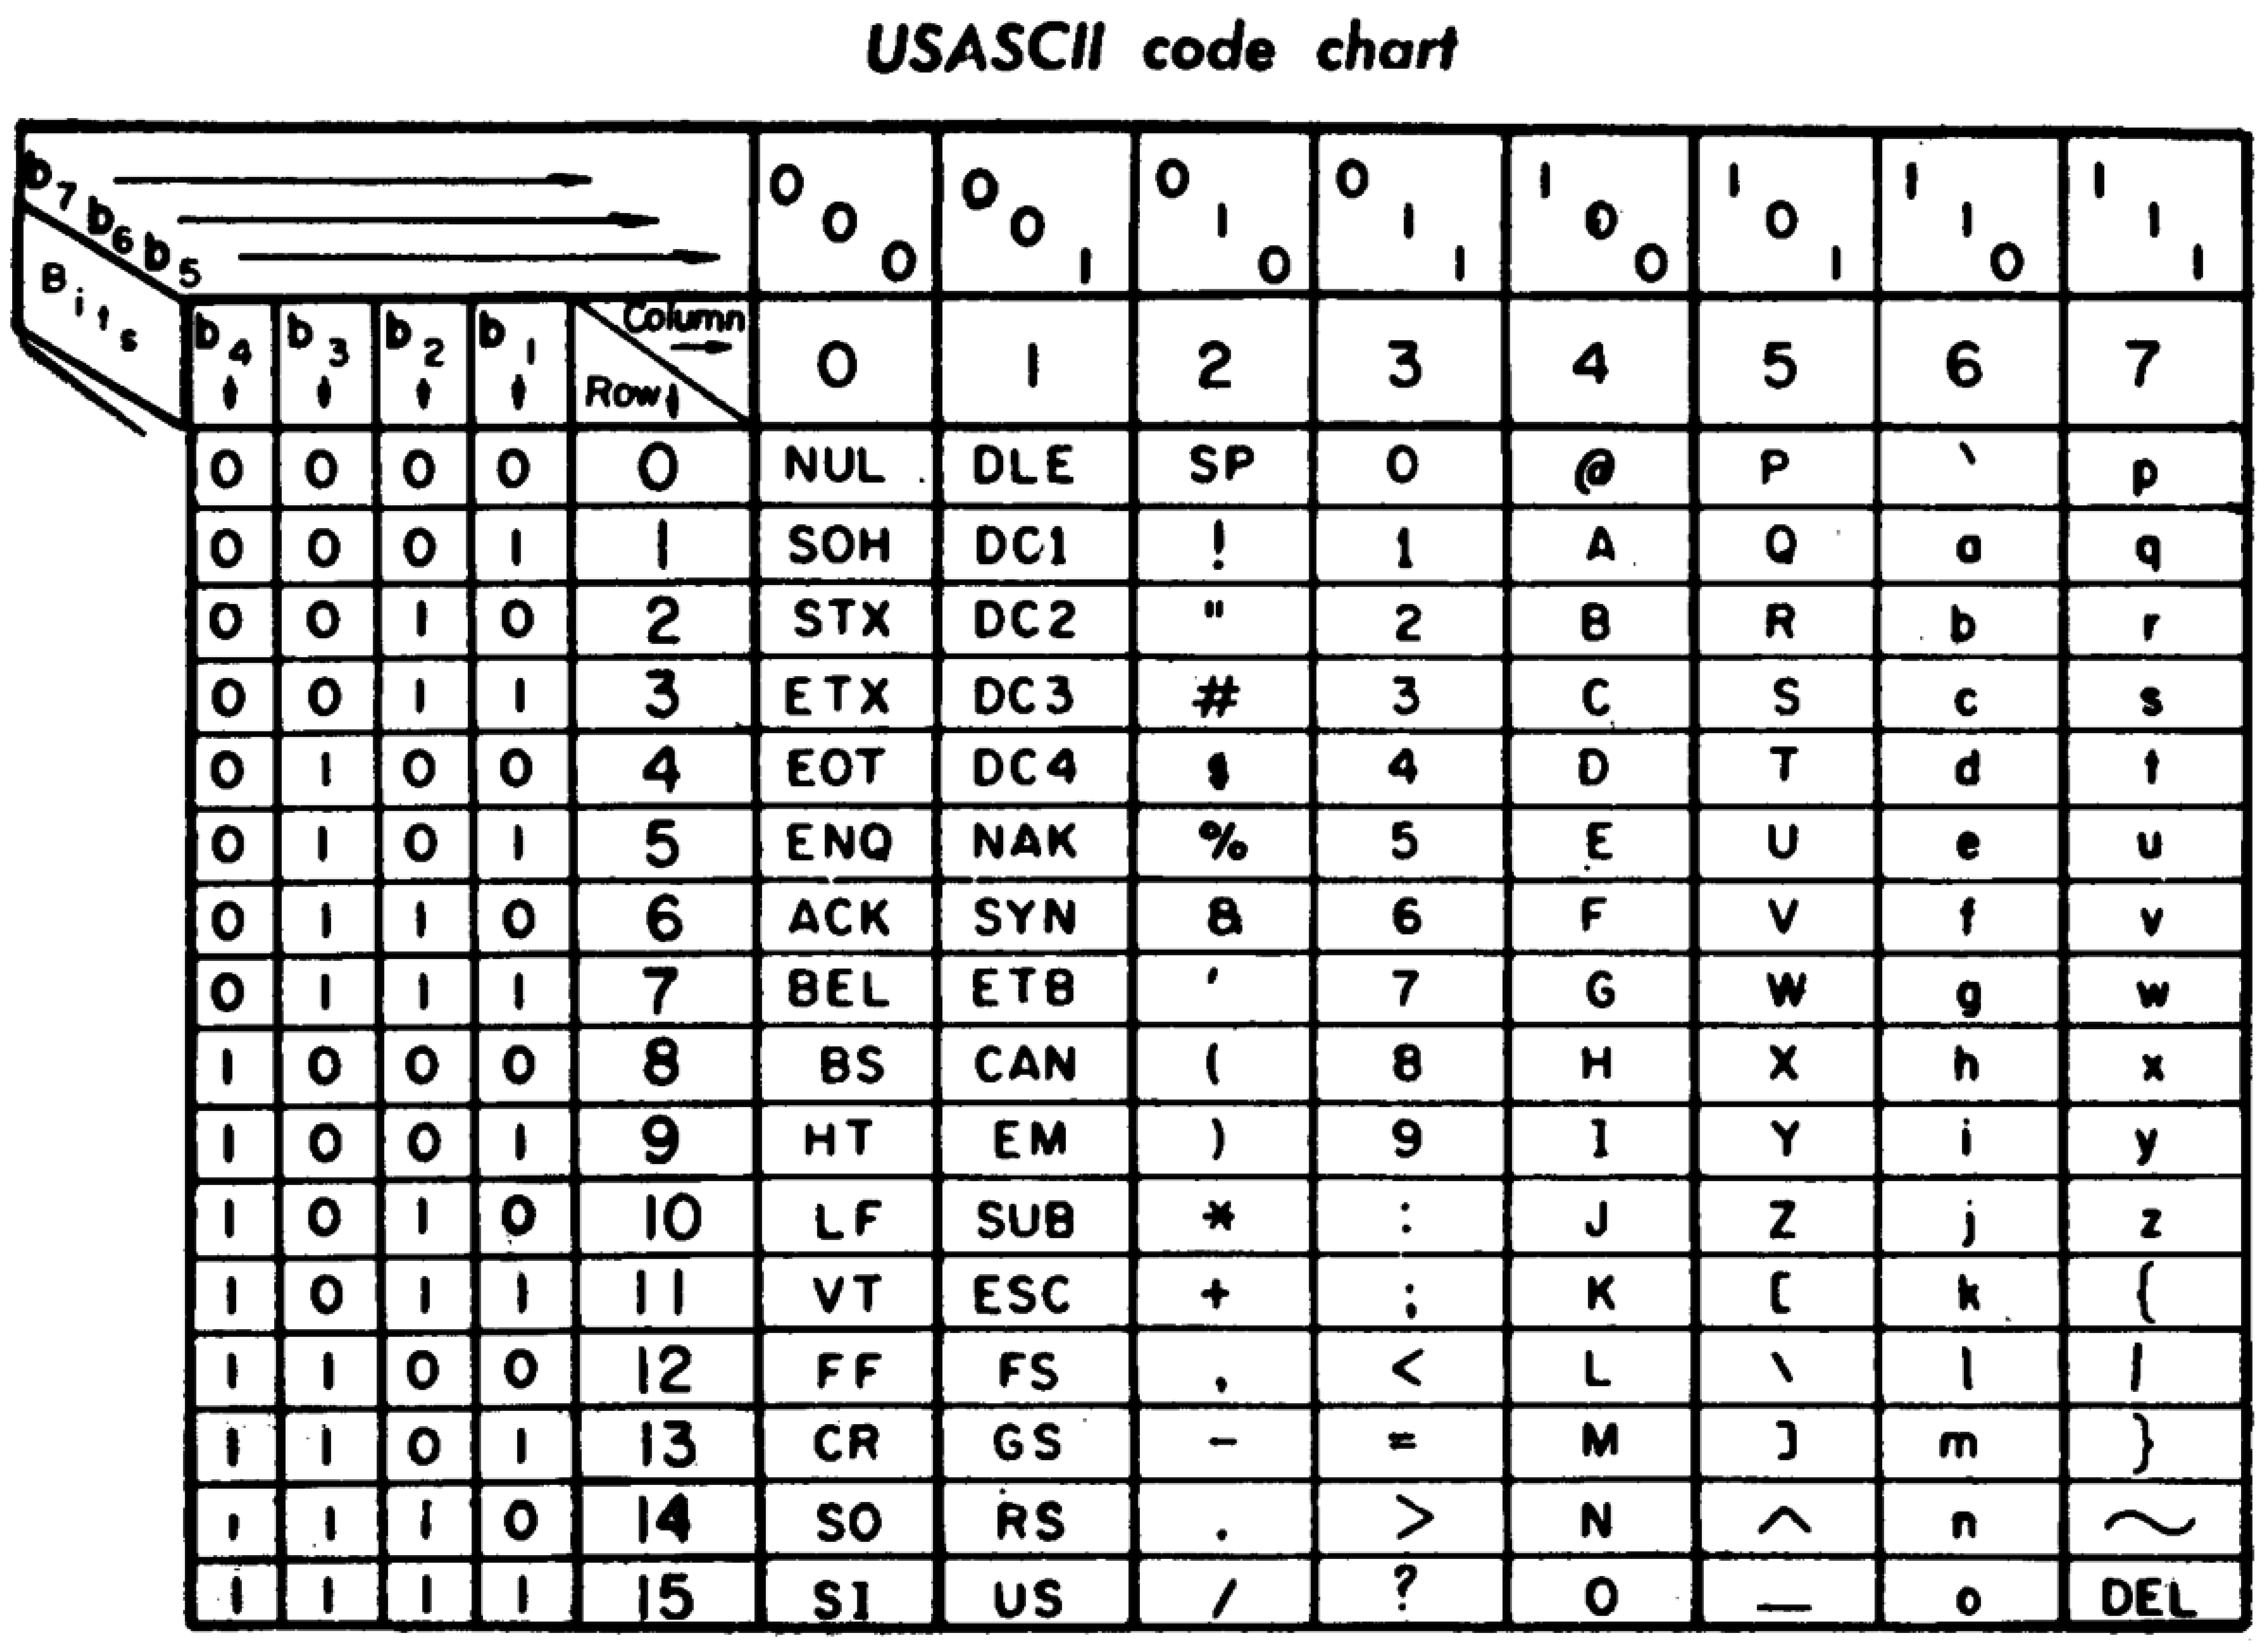
\includegraphics[scale=0.12]{images/US-ASCII_code_chart}

\footnotesize Source : https://en.wikipedia.org/wiki/ASCII\#/media/File:US-ASCII\_code\_chart.png
\end{center}

Par exemple, le caractère \pythoninline{'A'}, est le caractère numéro \mintinline{text}{100 0001}.

C'est-à-dire : \texttt{1}$\times2^6+$\texttt{0}$\times2^5+\ldots+$\texttt{0}$\times2^1+$\texttt{1}$\times2^0=65$ en décimal. 

Le tableau permet d'en lire l'écriture hexadécimale : \texttt{41}.

On peut vérifier par le calcul : \texttt{4}$\times16^1+$\texttt{1}$\times16^0=65$.

\medskip

Comme l'ASCII est la base de notre codage actuel, on obtient donc << A >> indifféremment par \pythoninline{'A'} ou \pythoninline{chr(65)} ou \pythoninline{chr(0x41)} ou encore \pythoninline{chr(0b1000001)}, et son code par \pythoninline{ord('A')}.

\section{Formats ISO}

L'amélioration de la fiabilité des transmissions et les besoins des européens, par exemple d'accentuer les lettres, ont abouti à l'utilisation du 8$^\text{ème}$ bit et donc à doubler le nombre de caractères codés. 
	
\Cours{{\bfseries latin-1}

\medskip C'est la norme ISO 8859-1 pour l'encodage des caractères. Elle contient les caractères accentués utilisés dans les langues latines.
}

On peut citer également :

\begin{itemize}
	\item l'ISO 8859-7 qui contient les caractères grecs.
    \item l'ISO 8859-15 ou latin 9, presque identique au latin 1 à 8 caractères près (le latin 9 contient par exemple les caractères œ, Œ et € qui ne sont pas dans la table latin 1).
\end{itemize}
	
L'encodage utilisé ne fait pas partie du contenu des fichier textes. Si on se trompe sur l'encodage utilisé, certains caractères seront donc mal interprétés. On voit encore apparaître des caractères sur des pages ou courriels dont l'encodage est mal spécifié. La phrase << C'est très raté ! >> par exemple devient << C'est très raté ! >>.

\section{Format Unicode}

\date{1990} Apparaît la norme Unicode, codée sur 2 octets (16 bits), pour réunir tous les caractères dans une seule table. On peut l'utiliser pour notre \pythoninline{'A'} :\pythoninline{'\u0041'}.

\medskip

Cette norme est encore en construction aujourd'hui, et contient actuellement plus de \np{135000} symboles codé sur 21 bits. Le code unicode n'est pas utilisé directement comme encodage de fichiers (sous peine de voir la taille des fichiers texte multipliée par 3). Ce sont des encodages comme UTF-8 qui permettent d'utiliser Unicode. 

\Cours{{\bfseries UTF-8}

\medskip C'est un encodage des caractères sur un seul octet, qui utilise des séquences d'échappement pour accéder à d'autres parties de la table. En UTF-8, tous les caractères n'occupent donc pas la même place. Certains sont codés sur 1 octet, et d'autres sur 2 à 4 octets.
} 

Pour expliquer le problème << C'est très raté ! >>, regardons comment est encodé << è >> :

\pythoninline{'è'.encode('utf8')} donne \pythoninline{b'\xc3\xa8'}.

On voit que le caractère d'échappement a le code hexadécimal : \texttt{C3}.

S'il n'était pas considéré comme échappement il serait \pythoninline{chr(0xc3)} qui donne \pythoninline{Ã}

\medskip

Et pour le << é >> ? 

\pythoninline{'é'.encode('utf8')} donne \pythoninline{b'\xc3\xa9'}. C'est le même échappement.

\medskip

Pour le << € >> il faut aller plus loin, l'échappement est différent : 

\pythoninline{'€'.encode('utf8')} donne \pythoninline{b'\xe2\x82\xac'}.

\medskip

Actuellement, la bonne pratique est d'utiliser UTF-8 dès que c'est possible.

\begin{minted}{python3}
# Supposons que fichier.txt soit encodé en latin1 !
with open('fichier.txt', encoding="latin1") as fichier :
    text = fichier.read()
with open('fichier.txt', mode="w", encoding="utf8") as fichier :
    fichier.write(text)
# Le problème est réglé.
\end{minted}